% Shared TikZ helpers --- layouts seguros (sin solapes)
\usetikzlibrary{arrows.meta,positioning,shapes.geometric,calc}

\tikzset{
  box/.style={
    draw=ieblue, rounded corners=3pt, align=center,
    fill=soft, font=\scriptsize, inner sep=5pt,
    minimum height=8.5mm, text depth=0.3em
  },
  boxdark/.style={
    draw=ieblue, rounded corners=3pt, align=center,
    fill=ieblue, text=white, font=\scriptsize\bfseries, inner sep=5pt,
    minimum height=8.5mm, text depth=0.3em
  },
  arr/.style={-{Latex}, thick, ieblue},
  pill/.style={
    draw=ieblue, rounded corners=8pt, fill=white,
    font=\scriptsize\bfseries, inner sep=4pt
  }
}

% Pipeline horizontal con anchos fijos y hueco para flechas
\newcommand{\PipelineFive}[5]{%
\begin{center}
\begin{tikzpicture}
  \node[box, text width=1.85cm] (a) {#1};
  \node[box, text width=1.85cm, right=0.55cm of a] (b) {#2};
  \node[box, text width=1.85cm, right=0.55cm of b] (c) {#3};
  \node[box, text width=1.85cm, right=0.55cm of c] (d) {#4};
  \node[boxdark, text width=1.85cm, right=0.55cm of d] (e) {#5};
  \draw[arr] (a) -- (b);
  \draw[arr] (b) -- (c);
  \draw[arr] (c) -- (d);
  \draw[arr] (d) -- (e);
\end{tikzpicture}
\end{center}%
}

% Encaje Pedro / Mario con minipages (evita solapes TikZ)
\newcommand{\FitDual}[4]{%
\noindent
\begin{minipage}[t]{0.48\textwidth}
\centering
\begin{tikzpicture}\node[circle, draw=ieblue, fill=blue!12, minimum size=1cm, font=\small\bfseries]{Pedro};\end{tikzpicture}\\[0.25em]
\begin{beamercolorbox}[wd=\textwidth,rounded=true,sep=4pt]{block body}
\scriptsize #1\\[0.35em]\textbf{Afinidad: #3/10}
\end{beamercolorbox}
\end{minipage}\hfill
\begin{minipage}[t]{0.48\textwidth}
\centering
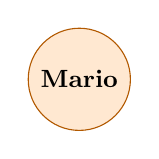
\begin{tikzpicture}\node[circle, draw=orange!70!black, fill=orange!18, minimum size=1cm, font=\small\bfseries]{Mario};\end{tikzpicture}\\[0.25em]
\begin{beamercolorbox}[wd=\textwidth,rounded=true,sep=4pt]{block body}
\scriptsize #2\\[0.35em]\textbf{Afinidad: #4/10}
\end{beamercolorbox}
\end{minipage}%
}

% Pros / contras con minipages
\newcommand{\ProCon}[2]{%
\noindent
\begin{minipage}[t]{0.48\textwidth}
\begin{beamercolorbox}[wd=\textwidth,rounded=true,sep=5pt]{block body}
\textcolor{good}{\textbf{Lo bueno}}\\[0.3em]
\scriptsize #1
\end{beamercolorbox}
\end{minipage}\hfill
\begin{minipage}[t]{0.48\textwidth}
\begin{beamercolorbox}[wd=\textwidth,rounded=true,sep=5pt]{block body}
\textcolor{bad}{\textbf{Lo malo}}\\[0.3em]
\scriptsize #2
\end{beamercolorbox}
\end{minipage}%
}

% Temario vs extensión
\newcommand{\MethodsSplit}[2]{%
\noindent
\begin{minipage}[t]{0.48\textwidth}
\begin{beamercolorbox}[wd=\textwidth,rounded=true,sep=5pt]{block body}
\textbf{Del curso}\\[0.25em]\scriptsize #1
\end{beamercolorbox}
\end{minipage}\hfill
\begin{minipage}[t]{0.48\textwidth}
\begin{beamercolorbox}[wd=\textwidth,rounded=true,sep=5pt]{block title}
\textbf{Más allá del temario}\\[0.15em]
\end{beamercolorbox}
\begin{beamercolorbox}[wd=\textwidth,rounded=true,sep=5pt]{block body}
\scriptsize #2
\end{beamercolorbox}
\end{minipage}%
}

\newcommand{\Verdict}[2]{%
\begin{center}
\begin{tikzpicture}
  \node[boxdark, text width=0.90\textwidth, align=center, font=\normalsize] {
    \textbf{\large #1}\\[0.35em]
    \normalfont\normalsize #2
  };
\end{tikzpicture}
\end{center}%
}

\newcommand{\ScoreBar}[3]{%
\noindent\begin{tikzpicture}
  \node[anchor=west, font=\scriptsize, text width=2.3cm] at (0,0) {#1};
  \fill[black!10] (2.4, -0.12) rectangle (6.6, 0.22);
  \fill[#3] (2.4, -0.12) rectangle ({2.4+#2*0.42}, 0.22);
  \node[font=\scriptsize\bfseries, anchor=west] at (6.75,0.05) {#2};
\end{tikzpicture}\par\vspace{0.1em}%
}

% Cabecera de opción sin solapes
\newcommand{\OptionHeader}[3]{%
\begin{center}
\begin{tikzpicture}
  \node[boxdark, text width=4.0cm] (a) {#1};
  \node[pill, right=0.5cm of a] (b) {#2};
\end{tikzpicture}
\end{center}
\vspace{0.35em}
\begin{block}{En una frase}
#3
\end{block}%
}
